\documentclass[12pt,a4paper]{amsart}

\usepackage[T1]{fontenc}
\usepackage[utf8]{inputenc}
\usepackage[english]{babel}
\usepackage{amsmath,amssymb,amsthm}
\usepackage{mathtools}
\usepackage{tikz}
\usepackage{geometry}
\usepackage[hidelinks]{hyperref}
\usetikzlibrary{arrows.meta,calc,fit,positioning,decorations.pathreplacing}
\geometry{margin=2.5cm}

\theoremstyle{definition}
\newtheorem{definition}{Definition}[section]

\theoremstyle{plain}
\newtheorem{lemma}[definition]{Lemma}
\newtheorem{proposition}[definition]{Proposition}
\newtheorem{theorem}[definition]{Theorem}

\newcommand{\len}[1]{\ell(#1)}
\newcommand{\dist}[3]{d_{#1}(#2,#3)}

\title{Structural properties of semi-cutting sets}
\author{}
\date{}
\keywords{semi-cutting sets, shortest paths, graph contraction, terminal distances, geodesic transversals}

\begin{document}

\begin{abstract}
Let $G=(V,E)$ be a finite simple undirected graph, let $T\subseteq V$, and let $F\subseteq E$. We call $F$ \emph{semi-cutting} for $T$ if $\dist{G}{u}{w}<\dist{G\setminus F}{u}{w}$ for every two distinct terminals $u,w\in T$. We prove the sharp lower bound $|F|\ge |T|-1$ for every semi-cutting set. The proof is entirely structural. We first characterize semi-cutting sets as edge transversals of terminal geodesics, then show that the property is preserved under contracting the closed neighborhood of a terminal not incident to $F$, and finally combine this with a terminal-deletion lemma in a lexicographic induction on $(|T|,|V|)$.
\end{abstract}

\maketitle

\section{Introduction}

Throughout the paper, graphs are finite, simple, and undirected. In particular, loops and parallel edges are excluded from the outset, and every contracted graph is understood in the usual simple-graph sense: loops are discarded and parallel edges are identified. For a graph $G=(V,E)$, a terminal set $T\subseteq V$, and an edge set $F\subseteq E$, we say that $F$ is \emph{semi-cutting} for $T$ if $\dist{G}{u}{w}<\dist{G\setminus F}{u}{w}$ for every two distinct terminals $u,w\in T$. Distances take values in $\mathbb{N}_0\cup\{\infty\}$, ordered by $n<\infty$ for every $n\in\mathbb{N}_0$.

The definition imposes no global restriction on the ambient graph. If some terminal pair already has infinite distance in $G$, then the inequality $\dist{G}{u}{w}<\dist{G\setminus F}{u}{w}$ becomes $\infty<\infty$, which is impossible. Thus the relevant terminal pairs are automatically joined in the original graph, but no connectivity assumption is made on $G$ itself.

Semi-cutting sets are related to two classical distance questions. When $|T|=2$, the condition says exactly that every geodesic between the prescribed terminals meets $F$, so the notion is close to the vital-link and vital-edge questions studied by Corley and Sha~\cite{corley-sha}, Malik, Mittal, and Gupta~\cite{malik-mittal-gupta}, and Nardelli, Proietti, and Widmayer~\cite{nardelli-proietti-widmayer}. For larger terminal sets, multiterminal cuts~\cite{dahlhaus1994} provide a natural comparison object: every multiterminal cut is semi-cutting whenever the original terminal distances are finite, but a semi-cutting set need not disconnect any terminal pair. We return to these relations in Section~\ref{sec:related}.

The main result is the sharp lower bound $|F|\ge |T|-1$. The proof is deliberately modular. Section~2 fixes notation and proves the auxiliary facts used later, including a complete geodesic characterization of the semi-cutting property. Section~3 establishes the contraction step and isolates the auxiliary terminal-deletion lemma that drives the second branch of the induction. Section~4 then gives the main theorem.

The bound is attained. For every integer $k\ge 2$, let $G$ be the path with vertex set $\{v_0,v_1,\dots,v_{2k-2}\}$ and edge set $\bigl\{\{v_i,v_{i+1}\}: i=0,\dots,2k-3\bigr\}$. Put $T=\{v_0,v_2,\dots,v_{2k-2}\}$ and $F=\bigl\{\{v_{2i},v_{2i+1}\}: i=0,\dots,k-2\bigr\}$. Then $|F|=|T|-1$, and after deleting $F$ each connected component contains exactly one terminal. Hence every terminal-terminal distance increases from a finite value in $G$ to $\infty$ in $G\setminus F$. Figure~\ref{fig:semi-cut-example} shows the case $k=3$.

\begin{figure}[htbp]
\centering
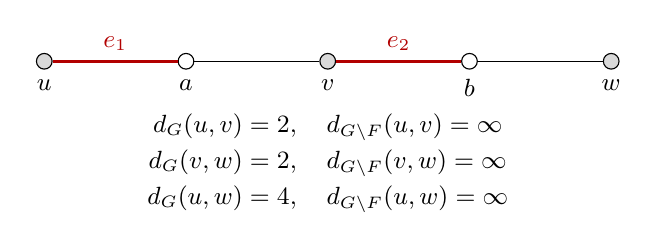
\begin{tikzpicture}[scale=1, every node/.style={font=\small}]
  \node[circle,draw,inner sep=2pt,fill=gray!30,label=below:$u$] (u) at (0,0) {};
  \node[circle,draw,inner sep=2pt,fill=white,label=below:$a$]   (a) at (1.8,0) {};
  \node[circle,draw,inner sep=2pt,fill=gray!30,label=below:$v$] (v) at (3.6,0) {};
  \node[circle,draw,inner sep=2pt,fill=white,label=below:$b$]   (b) at (5.4,0) {};
  \node[circle,draw,inner sep=2pt,fill=gray!30,label=below:$w$] (w) at (7.2,0) {};
  \draw[very thick,red!70!black] (u) -- node[above]{$e_1$} (a);
  \draw (a) -- (v);
  \draw[very thick,red!70!black] (v) -- node[above]{$e_2$} (b);
  \draw (b) -- (w);
  \node[align=center] at (3.6,-1.3)
    {$\dist{G}{u}{v}=2,\quad \dist{G\setminus F}{u}{v}=\infty$\\[2pt]
     $\dist{G}{v}{w}=2,\quad \dist{G\setminus F}{v}{w}=\infty$\\[2pt]
     $\dist{G}{u}{w}=4,\quad \dist{G\setminus F}{u}{w}=\infty$};
\end{tikzpicture}
\caption{A sharp example with $T=\{u,v,w\}$ and $F=\{e_1,e_2\}$.}
\label{fig:semi-cut-example}
\end{figure}

\section{Definitions and Auxiliary Lemmas}

Let $G=(V,E)$ be a finite simple graph. Distances take values in $\mathbb{N}_0\cup\{\infty\}$.

\begin{definition}[Walks, paths, and distance]\label{def:paths-distance}
Let $u,w\in V$. A \emph{walk} from $u$ to $w$ is a sequence $P=(v_0,v_1,\dots,v_k)$, where $k\in\mathbb{N}_0$, $v_0=u$, $v_k=w$, and $\{v_{i-1},v_i\}\in E$ for every $i\in\{1,\dots,k\}$. Its length is $\len{P}\coloneqq k$. A \emph{path} is a walk with pairwise distinct vertices. For a path $P=(v_0,\dots,v_k)$, we write $V(P)\coloneqq \{v_0,\dots,v_k\}$ and $E(P)\coloneqq \bigl\{\{v_{i-1},v_i\}: i=1,\dots,k\bigr\}$.

The \emph{distance} $\dist{G}{u}{w}$ is the minimum length of a path from $u$ to $w$ in $G$ when such a path exists, and $\infty$ otherwise. A path $P$ from $u$ to $w$ is \emph{shortest} if $\len{P}=\dist{G}{u}{w}$.
\end{definition}

If $F\subseteq E$, we write $G\setminus F\coloneqq (V,E\setminus F)$ and
\[
V(F)\coloneqq \{v\in V:\ \exists\, e\in F \text{ such that } v\in e\}.
\]
For a vertex $v\in V$, its open and closed neighborhoods are $N(v)\coloneqq \{w\in V:\ \{v,w\}\in E\}$ and $N[v]\coloneqq N(v)\cup\{v\}$. If $P=(v_0,\dots,v_k)$ is a path and $0\le i\le j\le k$, then $P[v_i,v_j]\coloneqq (v_i,\dots,v_j)$.

\begin{definition}[Contraction of a non-empty vertex set]\label{def:contraction}
Let $\emptyset\neq W\subseteq V$ and let $w^\ast\notin V$ be a new vertex. Define $\pi_W\colon V\to (V\setminus W)\cup\{w^\ast\}$ by $\pi_W(v)=w^\ast$ for $v\in W$ and $\pi_W(v)=v$ for $v\notin W$. The contracted graph $G/W$ has vertex set $(V\setminus W)\cup\{w^\ast\}$ and edge set
\[
E(G/W)=\bigl\{\{\pi_W(x),\pi_W(y)\}: \{x,y\}\in E,\ \pi_W(x)\neq \pi_W(y)\bigr\}.
\]
If $e=\{x,y\}\in E$ and $\pi_W(x)\neq \pi_W(y)$, we write $e/W\coloneqq \{\pi_W(x),\pi_W(y)\}\in E(G/W)$. For $F\subseteq E$, we also put
\[
F/W\coloneqq \bigl\{\{\pi_W(x),\pi_W(y)\}: \{x,y\}\in F,\ \pi_W(x)\neq \pi_W(y)\bigr\}\subseteq E(G/W).
\]
\end{definition}

\begin{definition}[Semi-cutting set]\label{def:semi-cut}
Let $T\subseteq V$. An edge set $F\subseteq E$ is a \emph{semi-cutting set} for $T$ in $G$ if $\dist{G}{u}{w}<\dist{G\setminus F}{u}{w}$ for every pair of distinct vertices $u,w\in T$. The vertices of $T$ are the \emph{terminals}.
\end{definition}

\begin{lemma}[Walks can be shortened to paths]\label{lem:walk-to-path}
Let $u,w\in V$. Every walk from $u$ to $w$ contains a path from $u$ to $w$ of length at most the length of the walk.
\end{lemma}

\begin{proof}
Let $P=(v_0,\dots,v_k)$ be a walk from $u$ to $w$. If the vertices of $P$ are pairwise distinct, then $P$ is already a path. Otherwise choose indices $i<j$ with $v_i=v_j$. Removing the closed subwalk $(v_i,\dots,v_j)$ yields the shorter walk
\[
(v_0,\dots,v_i,v_{j+1},\dots,v_k),
\]
where the tail $(v_{j+1},\dots,v_k)$ is omitted when $j=k$. The resulting walk still starts at $u$ and ends at $w=v_j=v_i$. Repeating this operation while repeated vertices remain produces a path, and the length never increases.
\end{proof}

\begin{lemma}[Subpaths of shortest paths]\label{lem:subpath-shortest}
Let $P=(v_0,\dots,v_k)$ be a shortest path in $G$. If $0\le i<j\le k$, then the subpath $P[v_i,v_j]$ is a shortest path from $v_i$ to $v_j$ in $G$.
\end{lemma}

\begin{proof}
Assume that $P[v_i,v_j]$ is not shortest. Then there exists a path $Q$ from $v_i$ to $v_j$ with $\len{Q}<j-i$. Replacing the segment $P[v_i,v_j]$ inside $P$ by $Q$ gives a walk from $v_0$ to $v_k$ of length smaller than $\len{P}$. By Lemma~\ref{lem:walk-to-path}, that walk contains a $v_0$--$v_k$ path shorter than $P$, contradicting the choice of $P$.
\end{proof}

\begin{lemma}[Projection of walks under contraction]\label{lem:projected-walk}
Let $\emptyset\neq W\subseteq V$, and let $P=(v_0,\dots,v_k)$ be a walk in $G$. Apply $\pi_W$ to each vertex of $P$ and then delete every consecutive repetition. The resulting sequence is a walk in $G/W$ from $\pi_W(v_0)$ to $\pi_W(v_k)$, and its length is at most $k$.
\end{lemma}

\begin{proof}
Put $z_i\coloneqq \pi_W(v_i)$ for $i=0,\dots,k$. For every index $i\in\{1,\dots,k\}$, either $z_{i-1}=z_i$ or $\{z_{i-1},z_i\}\in E(G/W)$ by Definition~\ref{def:contraction}. Now delete from the sequence $(z_0,\dots,z_k)$ every term equal to its predecessor. Each deletion removes one step and never changes the first or the last term. Whenever two consecutive terms remain distinct, they come from some adjacent pair $z_{i-1},z_i$ with $\{z_{i-1},z_i\}\in E(G/W)$. Hence the reduced sequence is a walk in $G/W$, and its length is bounded above by $k$ because only deletions were performed.
\end{proof}

\begin{lemma}[Geodesic characterization of the semi-cutting property]\label{lem:geodesic-characterization}
Let $X\subseteq V$ and $M\subseteq E$. Then $M$ is a semi-cutting set for $X$ in $G$ if and only if, for every two distinct vertices $u,w\in X$, the distance $\dist{G}{u}{w}$ is finite and every shortest $u$--$w$ path in $G$ contains an edge of $M$.
\end{lemma}

\begin{proof}
Assume first that $M$ is semi-cutting for $X$. Let $u,w\in X$ be distinct. If $\dist{G}{u}{w}=\infty$, then Definition~\ref{def:semi-cut} yields the contradiction $\infty=\dist{G}{u}{w}<\dist{G\setminus M}{u}{w}\le \infty$. Thus $\dist{G}{u}{w}<\infty$. Now let $P$ be a shortest $u$--$w$ path in $G$. If $E(P)\cap M=\emptyset$, then $P$ is also a path in $G\setminus M$, so
\[
\dist{G\setminus M}{u}{w}\le \len{P}=\dist{G}{u}{w},
\]
again contradicting Definition~\ref{def:semi-cut}. Hence every shortest $u$--$w$ path meets $M$.

Conversely, assume that for every two distinct vertices $u,w\in X$, the distance $\dist{G}{u}{w}$ is finite and every shortest $u$--$w$ path in $G$ contains an edge of $M$. Fix such a pair $u,w$. If $u$ and $w$ are disconnected in $G\setminus M$, then $\dist{G\setminus M}{u}{w}=\infty>\dist{G}{u}{w}$. Otherwise let $Q$ be a shortest $u$--$w$ path in $G\setminus M$. Then $Q$ is also a path in $G$, hence $\len{Q}\ge \dist{G}{u}{w}$. Equality is impossible, because then $Q$ would be a shortest $u$--$w$ path in $G$ disjoint from $M$. Therefore $\dist{G\setminus M}{u}{w}=\len{Q}>\dist{G}{u}{w}$, so $M$ is semi-cutting for $X$.
\end{proof}

\section{Contraction and Terminal Deletion}

\begin{lemma}\label{lem:contraction-image-size}
Let $\emptyset\neq W\subseteq V$ and let $F\subseteq E$. Then $|F/W|\le |F|$.
\end{lemma}

\begin{proof}
Let $D\coloneqq \bigl\{e\in F:\ e/W \text{ is defined}\bigr\}$. The map $D\to F/W$, given by $e\mapsto e/W$, is surjective, so $|F/W|\le |D|\le |F|$.
\end{proof}

\begin{lemma}\label{lem:outside-edges}
Let $t\in V$, let $t^\prime\notin V$ be a new vertex, and let $G^\prime\coloneqq G/N[t]$. If $x,y\in V\setminus N[t]$ are distinct, then $\{x,y\}\in E(G^\prime)$ if and only if $\{x,y\}\in E(G)$; in that case $\{x,y\}/N[t]=\{x,y\}$.
\end{lemma}

\begin{proof}
If $\{x,y\}\in E(G)$, then Definition~\ref{def:contraction} gives $\{x,y\}\in E(G^\prime)$ and $\{x,y\}/N[t]=\{x,y\}$. Conversely, if $\{x,y\}\in E(G^\prime)$, then some edge $\{u,v\}\in E(G)$ satisfies $\{\pi_{N[t]}(u),\pi_{N[t]}(v)\}=\{x,y\}$. Since neither $x$ nor $y$ is $t^\prime$, both $u$ and $v$ lie outside $N[t]$, hence $\{u,v\}=\{x,y\}\in E(G)$.
\end{proof}

\begin{lemma}\label{lem:lifting-endpoint}
Let $t\in V$, let $t^\prime\notin V$ be a new vertex, and let $G^\prime\coloneqq G/N[t]$. Let $z\in V\setminus N[t]$, and let $P^\prime=(t^\prime,x_1,\dots,x_k)$ be a shortest path from $t^\prime$ to $z$ in $G^\prime$. Then there exists a vertex $v\in N(t)$ such that $P=(t,v,x_1,\dots,x_k)$ is a shortest path from $t$ to $z$ in $G$.
\end{lemma}

\begin{proof}
Since $z\neq t^\prime$, we have $k\ge 1$. The edge $\{t^\prime,x_1\}$ belongs to $E(G^\prime)$, so Definition~\ref{def:contraction} provides a vertex $v\in N[t]$ with $\{v,x_1\}\in E(G)$. Because $x_1\notin N[t]$, the choice $v=t$ is impossible, and therefore $v\in N(t)$. Every vertex $x_i$ lies outside $N[t]$, hence every edge $\{x_{i-1},x_i\}$ of $P^\prime$ is also an edge of $G$ by Lemma~\ref{lem:outside-edges}. Consequently $P=(t,v,x_1,\dots,x_k)$ is a path in $G$ and $\len{P}=\len{P^\prime}+1$.

Now let $R=(r_0,\dots,r_\ell)$ be any path from $t$ to $z$ in $G$. Since $z\notin N[t]$, the second vertex $r_1$ lies in $N(t)$ and $\ell\ge 2$. Apply Lemma~\ref{lem:projected-walk} to the tail $(r_1,\dots,r_\ell)$. Because $r_1\in N[t]$ and $r_\ell=z\notin N[t]$, the resulting walk in $G^\prime$ runs from $t^\prime$ to $z$ and has length at most $\ell-1$. Lemma~\ref{lem:walk-to-path} therefore yields a $t^\prime$--$z$ path in $G^\prime$ of length at most $\ell-1$. Hence $\dist{G^\prime}{t^\prime}{z}\le \ell-1=\len{R}-1$. Since $R$ was arbitrary, we obtain $\dist{G}{t}{z}\ge \dist{G^\prime}{t^\prime}{z}+1$.

On the other hand, $P$ is a $t$--$z$ path in $G$, so
\[
\dist{G}{t}{z}\le \len{P}=\len{P^\prime}+1=\dist{G^\prime}{t^\prime}{z}+1.
\]
The two inequalities imply $\dist{G}{t}{z}=\len{P}$, and thus $P$ is shortest.
\end{proof}

\begin{figure}[t]
\centering
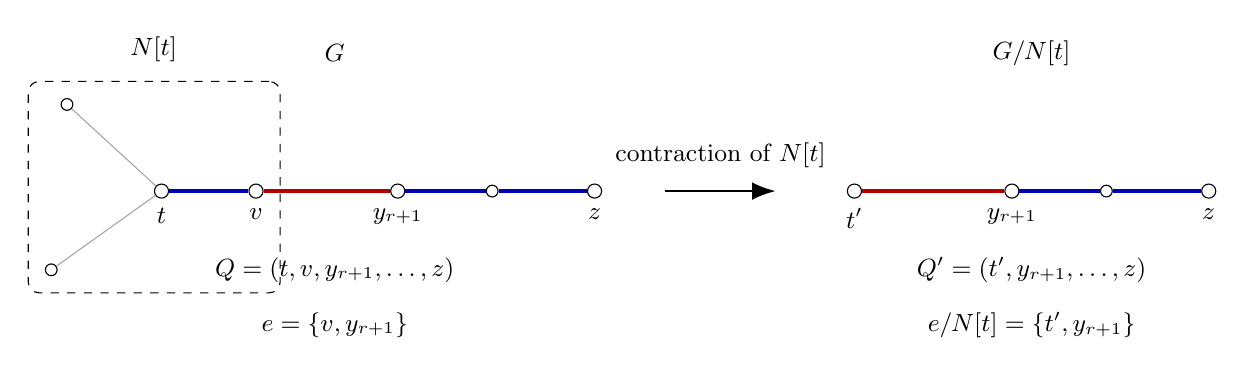
\begin{tikzpicture}[scale=1, every node/.style={font=\small}]
  \begin{scope}[xshift=0cm]
    \node[circle,draw,inner sep=1.5pt,fill=white] (a) at (-0.2,1.1) {};
    \node[circle,draw,inner sep=1.5pt,fill=white] (b) at (-0.4,-1.0) {};
    \node[circle,draw,inner sep=1.8pt,fill=white,label=below:$t$] (t) at (1.0,0.0) {};
    \node[circle,draw,inner sep=1.8pt,fill=white,label=below:$v$] (v) at (2.2,0.0) {};
    \node[circle,draw,inner sep=1.8pt,fill=white,label=below:$y_{r+1}$] (y1) at (4.0,0.0) {};
    \node[circle,draw,inner sep=1.5pt,fill=white] (y2) at (5.2,0.0) {};
    \node[circle,draw,inner sep=1.8pt,fill=white,label=below:$z$] (z) at (6.5,0.0) {};
    \draw[gray!70] (a)--(t) (b)--(t) (t)--(v);
    \draw[very thick,blue!70!black] (t)--(v)--(y1)--(y2)--(z);
    \draw[very thick,red!70!black] (v)--(y1);
    \node[draw,dashed,rounded corners,fit=(a)(b)(t)(v),inner sep=6pt] {};
    \node at (0.9,1.8) {$N[t]$};
    \node at (3.2,-1.0) {$Q=(t,v,y_{r+1},\dots,z)$};
    \node at (3.2,-1.7) {$e=\{v,y_{r+1}\}$};
    \node at (3.2,1.75) {$G$};
  \end{scope}

  \draw[-{Latex[length=3mm]},thick] (7.4,0) -- (8.8,0);
  \node at (8.1,0.45) {\small contraction of $N[t]$};

  \begin{scope}[xshift=9.8cm]
    \node[circle,draw,inner sep=1.8pt,fill=white,label=below:$t^\prime$] (tp) at (0.0,0.0) {};
    \node[circle,draw,inner sep=1.8pt,fill=white,label=below:$y_{r+1}$] (yp1) at (2.0,0.0) {};
    \node[circle,draw,inner sep=1.5pt,fill=white] (yp2) at (3.2,0.0) {};
    \node[circle,draw,inner sep=1.8pt,fill=white,label=below:$z$] (zp) at (4.5,0.0) {};
    \draw[very thick,blue!70!black] (tp)--(yp1)--(yp2)--(zp);
    \draw[very thick,red!70!black] (tp)--(yp1);
    \node at (2.25,-1.0) {$Q^\prime=(t^\prime,y_{r+1},\dots,z)$};
    \node at (2.25,-1.7) {$e/N[t]=\{t^\prime,y_{r+1}\}$};
    \node at (2.25,1.75) {$G/N[t]$};
  \end{scope}
\end{tikzpicture}
\caption{The suffix used in the lifting argument of Proposition~\ref{prop:contraction}.}
\label{fig:contraction}
\end{figure}

\begin{proposition}\label{prop:contraction}
Let $T\subseteq V$ and $F\subseteq E$. Assume that $F$ is a semi-cutting set for $T$ in $G$. Let $t\in T\setminus V(F)$ and let $t^\prime\notin V$ be a new vertex. Put $G^\prime\coloneqq G/N[t]$, $T^\prime\coloneqq (T\setminus\{t\})\cup\{t^\prime\}$, and $F^\prime\coloneqq F/N[t]$. Then $F^\prime$ is a semi-cutting set for $T^\prime$ in $G^\prime$.
\end{proposition}

\begin{proof}
We first show that no terminal of $T\setminus\{t\}$ lies in $N[t]$. Suppose that some $u\in T\setminus\{t\}$ belongs to $N[t]$. Then $\{t,u\}$ is the unique shortest $t$--$u$ path in $G$, so Lemma~\ref{lem:geodesic-characterization} forces $\{t,u\}\in F$. This contradicts $t\notin V(F)$. Therefore $T\setminus\{t\}\subseteq V\setminus N[t]$, and so $T^\prime\subseteq V(G^\prime)$.

Next we verify that every pair of distinct terminals in $T^\prime$ has finite distance in $G^\prime$. If $u,w\in T\setminus\{t\}$, then Lemma~\ref{lem:geodesic-characterization} yields a $u$--$w$ path in $G$; by Lemma~\ref{lem:projected-walk}, its projection contains a $u$--$w$ walk in $G^\prime$, and Lemma~\ref{lem:walk-to-path} turns this walk into a $u$--$w$ path in $G^\prime$. If one terminal is $t^\prime$ and the other is $z\in T\setminus\{t\}$, the same argument applied to any $t$--$z$ path in $G$ gives a $t^\prime$--$z$ path in $G^\prime$. By Lemma~\ref{lem:geodesic-characterization}, it now remains to show that every shortest path in $G^\prime$ between distinct terminals of $T^\prime$ meets $F^\prime$.

Let $u,w\in T^\prime$ be distinct, and let $P^\prime$ be a shortest $u$--$w$ path in $G^\prime$.

\smallskip\noindent
\textbf{Case 1: $t^\prime\notin V(P^\prime)$.}
Then every vertex of $P^\prime$ lies outside $N[t]$. Lemma~\ref{lem:outside-edges} shows that $P^\prime$ is also a path in $G$. It is shortest there as well. Indeed, if $R$ were a shorter $u$--$w$ path in $G$, then Lemma~\ref{lem:projected-walk} would produce a $u$--$w$ walk in $G^\prime$ of length at most $\len{R}<\len{P^\prime}$, and Lemma~\ref{lem:walk-to-path} would then yield a shorter $u$--$w$ path in $G^\prime$, contrary to the choice of $P^\prime$. Since $u,w\in T\setminus\{t\}\subseteq T$, Lemma~\ref{lem:geodesic-characterization} gives an edge $g\in E(P^\prime)\cap F$. Both ends of $g$ lie outside $N[t]$, so Lemma~\ref{lem:outside-edges} implies $g/N[t]=g\in F^\prime$.

\smallskip\noindent
\textbf{Case 2: $t^\prime\in V(P^\prime)$.}
Because the endpoints of $P^\prime$ play symmetric roles, we may write $P^\prime=(y_0,\dots,y_m)$ with $y_r=t^\prime$ for some $r<m$. Put $z\coloneqq y_m\in T^\prime\setminus\{t^\prime\}=T\setminus\{t\}$ and $Q^\prime\coloneqq P^\prime[y_r,y_m]$. By Lemma~\ref{lem:subpath-shortest}, the path $Q^\prime$ is shortest from $t^\prime$ to $z$ in $G^\prime$. Lemma~\ref{lem:lifting-endpoint} therefore yields a vertex $v\in N(t)$ such that
\[
Q=(t,v,y_{r+1},\dots,y_m)
\]
is a shortest path from $t$ to $z$ in $G$.

Since $t,z\in T$, Lemma~\ref{lem:geodesic-characterization} shows that $E(Q)\cap F\neq\emptyset$. The first edge $\{t,v\}$ of $Q$ does not belong to $F$, because $t\notin V(F)$. Choose $f\in E(Q)\cap F$. If $f=\{v,y_{r+1}\}$, then $f/N[t]=\{t^\prime,y_{r+1}\}$ is the first edge of $Q^\prime$. Otherwise $f=\{y_i,y_{i+1}\}$ for some $i\in\{r+1,\dots,m-1\}$, and both ends of $f$ lie outside $N[t]$; then Lemma~\ref{lem:outside-edges} gives $f/N[t]=f\in E(Q^\prime)$. In either situation, $f/N[t]\in E(Q^\prime)\subseteq E(P^\prime)$ and $f/N[t]\in F^\prime$.

Thus every shortest path between distinct terminals of $T^\prime$ intersects $F^\prime$. Lemma~\ref{lem:geodesic-characterization} completes the proof.
\end{proof}

\begin{figure}[t]
\centering
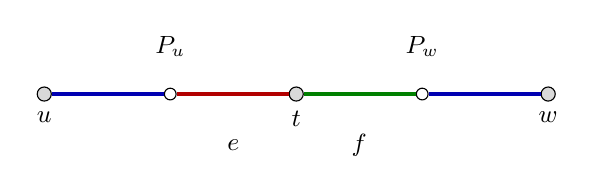
\begin{tikzpicture}[scale=1, every node/.style={font=\small}]
  \node[circle,draw,inner sep=1.8pt,fill=gray!30,label=below:$u$] (u) at (0,0) {};
  \node[circle,draw,inner sep=1.5pt,fill=white] (x) at (1.6,0) {};
  \node[circle,draw,inner sep=1.8pt,fill=gray!30,label=below:$t$] (t) at (3.2,0) {};
  \node[circle,draw,inner sep=1.5pt,fill=white] (y) at (4.8,0) {};
  \node[circle,draw,inner sep=1.8pt,fill=gray!30,label=below:$w$] (w) at (6.4,0) {};
  \draw[very thick,blue!70!black] (u)--(x)--(t)--(y)--(w);
  \draw[very thick,red!70!black] (x)--(t);
  \draw[very thick,green!50!black] (t)--(y);
  \node at (1.6,0.6) {$P_u$};
  \node at (4.8,0.6) {$P_w$};
  \node at (2.4,-0.65) {$e$};
  \node at (4.0,-0.65) {$f$};
\end{tikzpicture}
\caption{If a shortest $u$--$w$ path uses the edge $e$ incident with $t$, then the opposite subpath still witnesses an edge of $F\setminus\{e\}$. Here $t$ is removed only from the terminal set, not from the graph.}
\label{fig:split-path}
\end{figure}

\begin{lemma}[Deleting one terminal together with one incident edge]\label{lem:terminal-deletion}
Let $T\subseteq V$ and $F\subseteq E$. Assume that $F$ is a semi-cutting set for $T$ in $G$. Let $t\in T$, and let $e\in F$ be an edge incident with $t$. Put $T^-\coloneqq T\setminus\{t\}$ and $F^-\coloneqq F\setminus\{e\}$. Then $F^-$ is a semi-cutting set for $T^-$ in $G$.
\end{lemma}

\begin{proof}
If $|T^-|\le 1$, the statement is vacuous. Assume from now on that $|T^-|\ge 2$. By Lemma~\ref{lem:geodesic-characterization}, every two distinct vertices of $T^-$ have finite distance in $G$. It therefore suffices to prove that every shortest path between two distinct vertices of $T^-$ contains an edge of $F^-$.

Take distinct vertices $u,w\in T^-$, and let $P$ be a shortest $u$--$w$ path in $G$. Since $u,w\in T$, Lemma~\ref{lem:geodesic-characterization} gives $E(P)\cap F\neq\emptyset$. If $e\notin E(P)$, then already $E(P)\cap F^-\neq\emptyset$. Suppose now that $e\in E(P)$. Write $P=(v_0,\dots,v_m)$ and let $v_j=t$. Because $u,w\neq t$, we have $0<j<m$. Put $P_u\coloneqq (v_0,\dots,v_j)$ and $P_w\coloneqq (v_j,\dots,v_m)$, as in Figure~\ref{fig:split-path}. By Lemma~\ref{lem:subpath-shortest}, both $P_u$ and $P_w$ are shortest paths, respectively for the pairs $(u,t)$ and $(t,w)$.

Exactly one of the two subpaths $P_u$ and $P_w$ contains the edge $e$. Let $R$ be the other one. Then $R$ is a shortest path whose endpoints are $t$ and one of the terminals $u,w$, and $e\notin E(R)$. Lemma~\ref{lem:geodesic-characterization} yields an edge $f\in E(R)\cap F$. Since $e\notin E(R)$, we have $f\neq e$, so $f\in F^-$. As $E(R)\subseteq E(P)$, it follows that $E(P)\cap F^-\neq\emptyset$.

Thus every shortest path between distinct terminals of $T^-$ meets $F^-$. Lemma~\ref{lem:geodesic-characterization} shows that $F^-$ is semi-cutting for $T^-$.
\end{proof}

\section{The Main Theorem}

\begin{theorem}\label{thm:main}
Let $G=(V,E)$ be a finite simple undirected graph, let $T\subseteq V$, and let $F\subseteq E$. If $F$ is a semi-cutting set for $T$ in $G$, then $|F|\ge |T|-1$.
\end{theorem}

\begin{proof}
For $(k,n)\in \mathbb{N}_0^2$, let $\mathcal{S}(k,n)$ be the statement that every simple graph $H$ on $n$ vertices, every terminal set $X\subseteq V(H)$ with $|X|=k$, and every semi-cutting set $M\subseteq E(H)$ for $X$ satisfy $|M|\ge k-1$. We prove $\mathcal{S}(k,n)$ for all $(k,n)$ by induction on $(k,n)$ with the lexicographic order.

If $k\le 1$, then $\mathcal{S}(k,n)$ is immediate, because $|M|\ge 0\ge k-1$.

Now fix $(k,n)$ with $k\ge 2$, and assume that $\mathcal{S}(k',n')$ holds for every $(k',n')\prec (k,n)$. Let $G=(V,E)$ be a simple graph on $n$ vertices, let $T\subseteq V$ have size $k$, and let $F\subseteq E$ be semi-cutting for $T$ in $G$. We prove that $|F|\ge k-1$.

\smallskip\noindent
\textbf{Case 1: $T\setminus V(F)\neq \emptyset$.}
Choose $t\in T\setminus V(F)$. Since $k\ge 2$, there exists a vertex $u\in T\setminus\{t\}$. By Lemma~\ref{lem:geodesic-characterization}, the distance $\dist{G}{t}{u}$ is finite, so some path from $t$ to $u$ exists and in particular $N(t)\neq\emptyset$. Hence $|N[t]|\ge 2$. Let $t^\prime\notin V$ be a new vertex, and define $G^\prime\coloneqq G/N[t]$, $T^\prime\coloneqq (T\setminus\{t\})\cup\{t^\prime\}$, and $F^\prime\coloneqq F/N[t]$. Proposition~\ref{prop:contraction} shows that $F^\prime$ is semi-cutting for $T^\prime$ in $G^\prime$. Moreover, $|T^\prime|=|T|=k$ and
\[
|V(G^\prime)|=|V|-|N[t]|+1\le n-1<n.
\]
Therefore $(|T^\prime|,|V(G^\prime)|)\prec (k,n)$, and the inductive hypothesis yields $|F^\prime|\ge |T^\prime|-1=k-1$. Lemma~\ref{lem:contraction-image-size} gives $|F^\prime|\le |F|$, so $|F|\ge k-1$.

\smallskip\noindent
\textbf{Case 2: $T\subseteq V(F)$.}
Choose any terminal $t\in T$. Since $t\in V(F)$, there exists an edge $e\in F$ incident with $t$. Put $T^-\coloneqq T\setminus\{t\}$ and $F^-\coloneqq F\setminus\{e\}$. By Lemma~\ref{lem:terminal-deletion}, the set $F^-$ is semi-cutting for $T^-$ in $G$. Because $|T^-|=k-1$, we have $(|T^-|,|V(G)|)\prec (k,n)$. The inductive hypothesis therefore yields
\[
|F^-|\ge |T^-|-1=k-2.
\]
Consequently $|F|=|F^-|+1\ge k-1$.

This completes the induction and proves the theorem.
\end{proof}

\section{Related Problems and Further Directions}\label{sec:related}

The path family from the introduction shows that Theorem~\ref{thm:main} is sharp. The first unresolved structural question is therefore the equality case: which triples $(G,T,F)$ satisfy $F$ semi-cutting for $T$ and $|F|=|T|-1$?

For two terminals, semi-cutting sets are exactly edge transversals of the family of geodesics between one prescribed pair of vertices. In that sense the notion is close to the vital-link and vital-edge literature initiated by Corley and Sha~\cite{corley-sha} and continued by Malik, Mittal, and Gupta~\cite{malik-mittal-gupta} and by Nardelli, Proietti, and Widmayer~\cite{nardelli-proietti-widmayer}. The common theme is the effect of deleting edges on shortest paths. The difference is conceptual: those works concentrate on one distinguished terminal pair, whereas a semi-cutting set must obstruct every geodesic between every two vertices of a prescribed terminal set.

For larger terminal sets, the nearest classical comparison is the multiterminal cut problem of Dahlhaus, Johnson, Papadimitriou, Seymour, and Yannakakis~\cite{dahlhaus1994}. There one asks for an edge set whose deletion separates each terminal from all the others. Semi-cutting is weaker: it requires only a strict increase of every terminal-terminal distance. Hence every multiterminal cut is semi-cutting whenever all original terminal distances are finite, but the converse fails because a semi-cutting set may leave all terminal pairs connected.

Lemma~\ref{lem:geodesic-characterization} also places semi-cutting sets inside the broader theory of geodesic transversals. On the vertex side, Harary, Loukakis, and Tsouros~\cite{harary-loukakis-tsouros} introduced the geodetic number, where one asks for a vertex set whose geodetic closure equals the whole graph. A closer comparison is provided by strong metric dimension: Oellermann and Peters-Fransen~\cite{oellermann-peters-fransen} related that parameter to mutually maximally distant pairs, and Peterin and Semani\v{s}in~\cite{peterin-semanisin} made explicit the link with maximal shortest paths cover. Manuel, Bre\v{s}ar, and Klav\v{z}ar~\cite{manuel-bresar-klavzar-transversal,manuel-bresar-klavzar-packing} studied transversal and packing questions for maximal geodesics. Semi-cutting sets differ from these parameters in two basic ways: they are edge sets rather than vertex sets, and they concern only those geodesics whose endpoints lie in a prescribed terminal set.

These comparisons suggest two natural directions. One is the structural description of the equality case in Theorem~\ref{thm:main}. The other is the study of minimum semi-cutting sets as edge transversals of the terminal-geodesic system determined by $T$.

\begin{thebibliography}{10}

\bibitem{diestel}
R.~Diestel,
\emph{Graph Theory},
6th ed., Graduate Texts in Mathematics 173, Springer, Heidelberg, 2025.

\bibitem{corley-sha}
H.~W. Corley, D.~Y. Sha,
\emph{Most vital links and nodes in weighted networks},
Operations Research Letters 1(4) (1982), 157--160.

\bibitem{malik-mittal-gupta}
K.~Malik, A.~K. Mittal, S.~K. Gupta,
\emph{The $k$ most vital arcs in the shortest path problem},
Operations Research Letters 8(4) (1989), 223--227.

\bibitem{nardelli-proietti-widmayer}
E.~Nardelli, G.~Proietti, P.~Widmayer,
\emph{A faster computation of the most vital edge of a shortest path},
Information Processing Letters 79(2) (2001), 81--85.

\bibitem{dahlhaus1994}
E.~Dahlhaus, D.~S. Johnson, C.~H. Papadimitriou, P.~D. Seymour, M.~Yannakakis,
\emph{The complexity of multiterminal cuts},
SIAM Journal on Computing 23(4) (1994), 864--894.

\bibitem{harary-loukakis-tsouros}
F.~Harary, E.~Loukakis, C.~Tsouros,
\emph{The geodetic number of a graph},
Mathematical and Computer Modelling 17(11) (1993), 89--95.

\bibitem{oellermann-peters-fransen}
O.~R. Oellermann, J.~Peters-Fransen,
\emph{The strong metric dimension of graphs and digraphs},
Discrete Applied Mathematics 155 (2007), 356--364.

\bibitem{manuel-bresar-klavzar-transversal}
P.~D. Manuel, B.~Bre\v{s}ar, S.~Klav\v{z}ar,
\emph{The geodesic-transversal problem},
Applied Mathematics and Computation 413 (2022), Art.~126621.

\bibitem{peterin-semanisin}
I.~Peterin, G.~Semani\v{s}in,
\emph{On the maximal shortest paths cover number},
Mathematics 9(14) (2021), Art.~1592.

\bibitem{manuel-bresar-klavzar-packing}
P.~D. Manuel, B.~Bre\v{s}ar, S.~Klav\v{z}ar,
\emph{Geodesic packing in graphs},
Applied Mathematics and Computation 459 (2023), Art.~128277.

\end{thebibliography}

\end{document}
